% !TEX root = ../popl-paper.tex

% \begin{figure}[ht]
% 	\begin{center}
% 	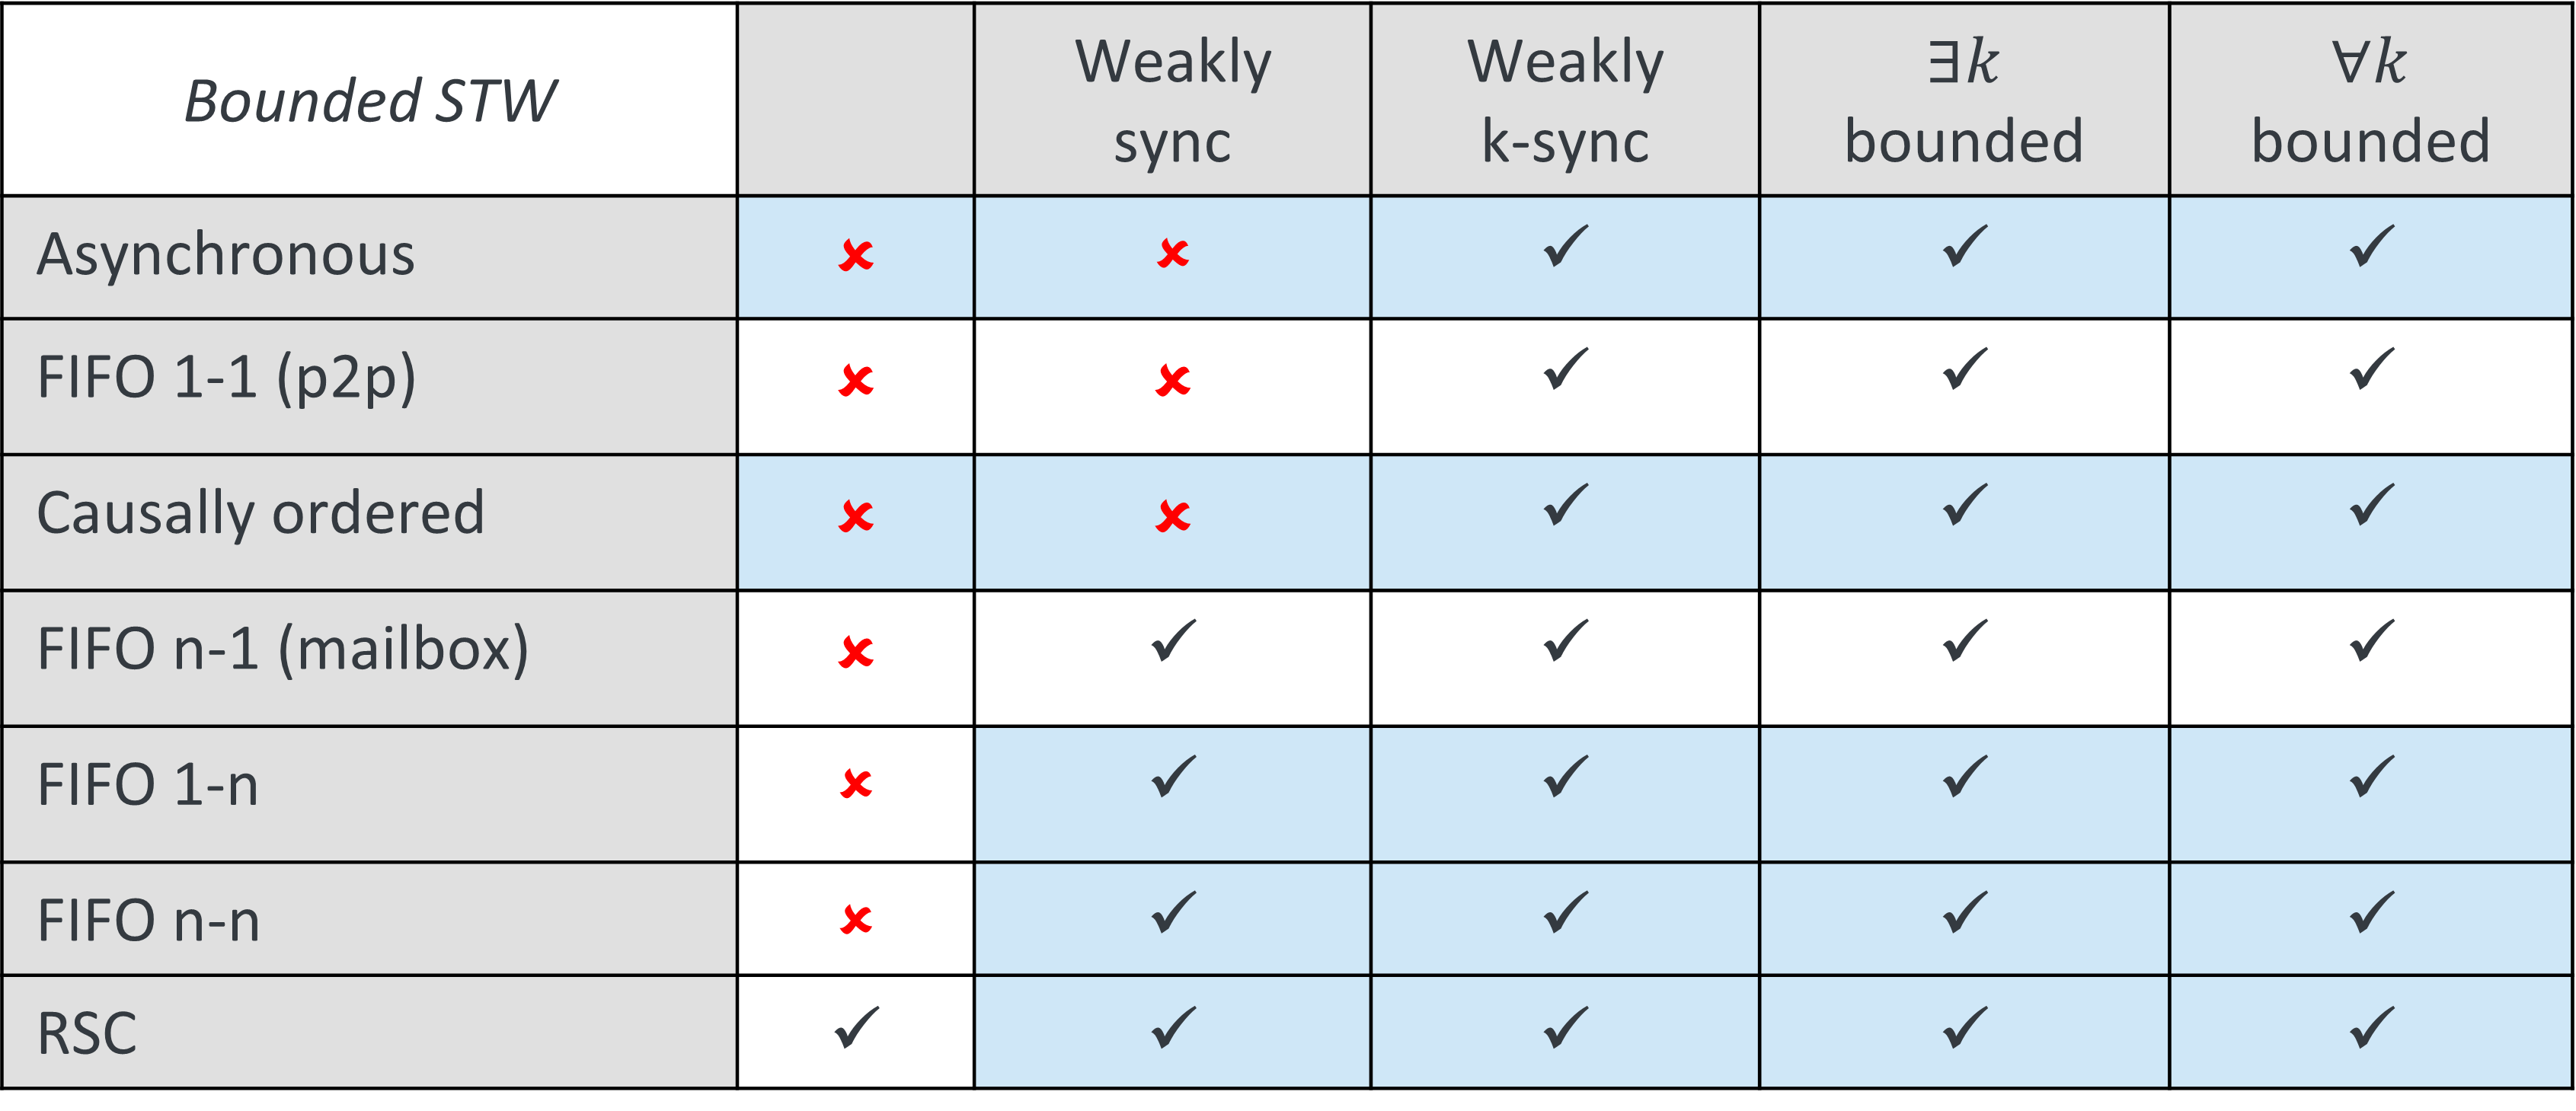
\includegraphics[width=10cm]{stw_bound}
% 	\end{center}
% \end{figure}


\begin{figure}[t]
		\begin{tabular}{| c | c | c|  c| c| }
			\hline
			& Weakly  & Weakly  & $\exists$k & $\forall$k  \\
			& sync & k-sync & bounded & bounded \\
			\hline \hline
			$\asy$ &  \xmark & \cmark & \cmark & \cmark \\
			\hline
			$\oneone$  & \xmark~[1] & \cmark~[1] & \cmark~[1] & \cmark~[1] \\
			\hline
			$\co$  & \xmark & \cmark & \cmark & \cmark \\
			\hline
			$\none$ & \cmark~[1] & \cmark~[1] & \cmark~[1] & \cmark~[1] \\
			\hline
			$\onen$ & \cmark & \cmark & \cmark & \cmark \\
			\hline
			$\nn$ & \cmark & \cmark & \cmark & \cmark \\
			\hline
		%	$\rsc$ & \cmark & \cmark & \cmark & \cmark & \cmark \\
		%	\hline
		\end{tabular}
		\caption{Table summarising the (un)decidability results for the synchronisability problems (each 
		combination of a communication model $\comsymb$ and a class $\aMSCclass$ of MSCs is a different 
		synchronisability problem). 
		The symbol \xmark\;stands for undecidability and unbounded special tree-width
		of $\comsymb\cap \aMSCclass$, whereas \cmark\;stands for decidability and bounded STW
		of $\comsymb\cap \aMSCclass$.  
		[1] indicates that the result was shown by Bollig~\emph{et al}~\cite{DBLP:conf/concur/BolligGFLLS21}.}
		\label{fig:stw-bound}
\end{figure}


In \cite{BolligFG21} the authors introduce a general framework based on MSO-logic and special treewidth (a graph property) that allows to derive decidability results for the \emph{synchronizability problem}. Roughly, the synchronizability problem consists in understanding whether all the behaviours/computations generated by a system have certain properties. The results in \cite{BolligFG21} hold for the $\oneone$ and the $\none$ communication models, which are referred to as p2p and mailbox, respectively. We show here that this framework can be effectively extended to all the 7 communication models that we considered.

\subsection{Special treewidth}

\emph{Special treewidth} \cite{Courcelle10},
is a graph measure that somehow indicates how close
a graph is to a tree (we may also use classical \emph{treewidth} instead).
This or similar measures are commonly employed in verification. For instance, treewidth and split-width have been used in \cite{MadhusudanP11} and \cite{DBLP:conf/concur/CyriacGK12,AiswaryaGK14}, respectively, to reason about graph behaviors generated by pushdown and queue systems.
%Here we apply it to reason about MSCs.
There are several ways to define the special treewidth of an MSC.
We adopt the following game-based definition from \cite{DBLP:journals/corr/abs-1904-06942}.

Adam and Eve play a turn based ``decomposition game'' on an MSC $\msc = (\Events, \procrel, \lhd, \lambda)$. $\msc$ is interpreted as a graph where nodes are the events and edges are represented by the $\procrel$ and the $\lhd$ relations.
Eve starts to play and does a move, which consists in the following steps:
\begin{enumerate}
	\item marking some events of $\msc$, resulting in the \emph{marked MSC fragment} $(M, U')$, where $U' \subseteq \Events$ is the subset of marked events,
	\item removing edges whose both endpoints are marked, in such a way that the resulting MSC is disconnected (i.e. there are at least two different connected components),
	\item splitting $(M, U)$ in $(M_1, U_1)$ and $(M_2, U_2)$ such that $M$ is the disjoint (unconnected) union of $M_1$ and $M_2$
	and marked nodes are inherited.
\end{enumerate}
Once Eve does her move, it is Adam's turn. Adam simply chooses one of the two marked MSC fragments, either $(M_1, U_1)$ or $(M_2, U_2)$. Now it is again Eve's turn, and she has to do a move on the marked MSC fragment that was chosen by Adam. The game continues in alternating turns between the two players until they reach a point where all the events on the current marked MSC fragment are marked.
For $k \in \N$, we say that the game is $k$-winning for Eve if she has a strategy that allows her, independently of Adam's moves, to end the game in a way that every marked MSC fragment visited during the game has at most $k+1$ marked events. The goal of Eve is to keep $k$ as low as possible. Fig.~\ref{fig:stw-ex} shows an example of a 3-winning game for the MSC in Fig.~\ref{fig:pp_ex}.

\newcommand{\CS}[2]{\mathsf{CS}_{(#1,#2)}}
\newcommand{\MSO}[2]{\mathsf{MSO}_{(#1,#2)}}
\newcommand{\LCPDL}[2]{\mathsf{LCPDL}_{(#1,#2)}}
\newcommand{\MSCpm}[2]{\mathsf{MSC}_{(#1,#2)}}
\newcommand{\mbMSCpm}[2]{\mathsf{MSC}_{(#1,#2)}^{\mathsf{mb}}}


\begin{fact}[\cite{DBLP:journals/corr/abs-1904-06942}]
	The special treewidth of an MSC is the least $k$ such that
	the associated game is $k$-winning for Eve.
\end{fact}

The set of MSCs whose special treewidth is at most $k$ is denoted by $\stwMSCs{k}$.

\begin{example}
	Let $\msc$ the MSC of the Fig.~\ref{fig:pp_ex}. In this example, we show that $\msc$ has a special treewidth  $\le 3$, since Eve is able to find a strategy that leads to a 3-winning game.  We use colors to mark events. Eve starts by marking 4 events. The edges whose both endpoints are marked can be removed (dotted edges in the figure) and the graph becomes disconnected. Eve then splits the graph in 2 and Adam has to choose.
	Suppose the Adam picks the subgraph with the red and yellow events already marked (top branch in the figure). Eve can mark the third event and, by doing so, the game ends.
	Suppose Adam chooses the subgraph with the blue and green events (bottom branch). Eve marks the two nodes in the bottom, removes 3 edges, and splits the graph in two. Note that one of the two subgraphs already has all events marked, so Adam is picks the other one (top branch).
	Eve simply marks the missing event and the game ends. This is a 3-winning game for Eve since, indipendently of Adam's choices, we have at most 4 marked event at each step.
\end{example}
% !TEX root = ../popl-paper.tex

\begin{figure}[t]
	\begin{center}
		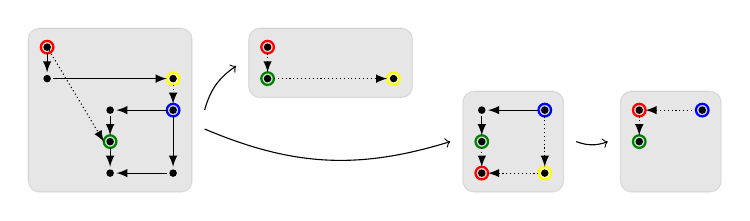
\begin{tikzpicture}[scale = .8]
			\begin{scope}
				\draw[gray,fill = gray, rounded corners, opacity=0.2] (-.3,.3) rectangle (2.3,-2.3);
				\draw[red, thick, fill = red!20] (0,0) circle (0.1);
				\draw[Green, thick, fill = Green!20] (1,-1.5) circle (0.1);
				\draw[Yellow, thick, fill = Yellow!20] (2,-.5) circle (0.1);
				\draw[blue, thick, fill = blue!20] (2,-1) circle (0.1);

				\draw[black, fill = black] (0,0) circle (.05);
				\draw[black, fill = black] (0,-.5) circle (.05);
				\draw[black, fill = black] (2,-.5) circle (.05);
				\draw[black, fill = black] (1,-1) circle (.05);
				\draw[black, fill = black] (2,-1) circle (.05);
				\draw[black, fill = black] (1,-1.5) circle (.05);
				\draw[black, fill = black] (1,-2) circle (.05);
				\draw[black, fill = black] (2,-2) circle (.05);

				\draw[>=latex, ->] (0,-.1) to (0, -.4);
				\draw[>=latex, ->,  densely dotted] (0,0) to (.9, -1.5);
				\draw[>=latex, ->] (.1,-.5) to (1.9, -.5);
				\draw[>=latex, ->,  densely dotted] (2,-.6) to (2, -.9);
				\draw[>=latex, ->] (1.9,-1) to (1.1, -1);
				\draw[>=latex, ->] (1,-1.1) to (1, -1.4);
				\draw[>=latex, ->] (1,-1.6) to (1, -1.9);
				\draw[>=latex, ->] (2,-1.1) to (2, -1.9);
				\draw[>=latex, ->] (1.9,-2) to (1.1, -2);

				\draw[->] (2.5,-1) to[bend left = 20] (3,-.3);
				\draw[->] (2.5,-1.3) to[bend right = 20] (6.4,-1.5);
				\draw[->] (8.4,-1.5) to[bend right = 20] (8.9,-1.5);


			\end{scope}
			\begin{scope}[shift = {(3.5,0)}]
				\draw[gray,fill = gray, rounded corners, opacity=0.2] (-.3,.3) rectangle (2.3,-.8);
				\draw[red, thick, fill = red!20] (0,0) circle (0.1);
				\draw[Green, thick, fill = Green!20] (0,-.5) circle (0.1);
				\draw[Yellow, thick, fill = Yellow!20] (2,-.5) circle (0.1);

				\draw[black, fill = black] (0,0) circle (.05);
				\draw[black, fill = black] (0,-.5) circle (.05);
				\draw[black, fill = black] (2,-.5) circle (.05);

				\draw[>=latex, ->, densely dotted	] (0,-.1) to (0, -.4);
				\draw[>=latex, ->, densely dotted	] (.1,-.5) to (1.9, -.5);
			\end{scope}
			\begin{scope}[shift = {(5.9,0)}]
				\draw[gray,fill = gray, rounded corners, opacity=0.2] (.7,-.7) rectangle (2.3,-2.3);
				\draw[red, thick, fill = red!20] (1,-2) circle (0.1);
				\draw[Green, thick, fill = Green!20] (1,-1.5) circle (0.1);
				\draw[Yellow, thick, fill = Yellow!20] (2,-2) circle (0.1);
				\draw[blue, thick, fill = blue!20] (2,-1) circle (0.1);

				\draw[black, fill = black] (1,-1) circle (.05);
				\draw[black, fill = black] (2,-1) circle (.05);
				\draw[black, fill = black] (1,-1.5) circle (.05);
				\draw[black, fill = black] (1,-2) circle (.05);
				\draw[black, fill = black] (2,-2) circle (.05);
				\draw[>=latex, ->] (1.9,-1) to (1.1, -1);
				\draw[>=latex, ->] (1,-1.1) to (1, -1.4);
				\draw[>=latex, ->,  densely dotted] (1,-1.6) to (1, -1.9);
				\draw[>=latex, ->,  densely dotted] (2,-1.1) to (2, -1.9);
				\draw[>=latex, ->,  densely dotted] (1.9,-2) to (1.1, -2);
			\end{scope}

			\begin{scope}[shift = {(8.4,0)}]
				\draw[gray,fill = gray, rounded corners, opacity=0.2] (.7,-.7) rectangle (2.3,-2.3);
				\draw[red, thick, fill = red!20] (1,-1) circle (0.1);
				\draw[Green, thick, fill = Green!20] (1,-1.5) circle (0.1);
				%\draw[Yellow, thick, fill = Yellow!20] (2,-2) circle (0.1);
				\draw[blue, thick, fill = blue!20] (2,-1) circle (0.1);

				\draw[black, fill = black] (1,-1) circle (.05);
				\draw[black, fill = black] (2,-1) circle (.05);
				\draw[black, fill = black] (1,-1.5) circle (.05);

				\draw[>=latex, ->,  densely dotted] (1.9,-1) to (1.1, -1);
				\draw[>=latex, ->,  densely dotted] (1,-1.1) to (1, -1.4);
				\end{scope}

		\end{tikzpicture}
	\end{center}
  \caption{Decomposition game for the MSC of Fig.~\ref{fig:pp_ex}. This is a 3-winning game for Eve.}
  \label{fig:stw-ex}
\end{figure}


\subsection{The synchronizability problem}

The synchronizability problem consists in understanding whether all the behaviours generated by a communicating system have a particular shape, i.e.  whether they are all included in a given set of MSCs $\Class$. A communicating system consists of processes, modeled as finite-state machines, that can exchange messages. A communicating system can use any of the communication models that we discussed. Given a system $\Sys$, let $\cL{\Sys}$ be the set of MSCs that represent all the possible behaviours of $\Sys$ when implementing a given communication model, where $\comsymb \in \{$$\asy, $ $\oneone, $ $\co, $ $\none, $ $\onen, $ $\nn, $ $\rsc\}$. Formally, the synchronizability problem is an inclusion problem, namely $\cL{\Sys} \subseteq \Class$. In \cite{BolligFG21} the authors show that, for $\comsymb = \oneone$ and $\comsymb = \none$, the synchronizability problem is decidable if $\Class$ is MSO-definable and special treewidth bounded (STW-bounded). In particular, among the classes $\Class$ that they considered, we will recall weakly synchronous, weakly k-synchronous, existentially $k$-bounded, and universally $k$-bounded MSCs. As shown in \cite{BolligFG21}, if we have a system $\Sys$ and a STW-bounded class $\Class$, then the model-checking problem\footnote{Given $\Procs$ and $\Msg$, a communicating system $\Sys$, an MSO sentence $\phi$, do we have $\cL{\Sys} \subseteq L(\phi)?$} for $\Sys$ becomes decidable if $L(S) \subseteq \Class$; this motivates the study of the synchronizability problem. Fig.~\ref{} shows the results about decidability of the synchronizability problem for each of these classes and all 7 communication models. Theorem~\ref{thm:sync} is the main result that allows to derive the decidability of the synchronizability problem ($SP$ in the following); Appendix~\ref{apx:sync} is entirely devoted to the proof of Theorem~\ref{thm:sync}.

\begin{restatable}{theorem}{thmsync}\label{thm:sync}
	Fix finite sets $\Procs$ and $\Msg$.
	Let $\comsymb \in \{$$\asy, $ $\oneone, $ $\co, $ $\none, $ $\onen, $ $\nn\}$ and let $\Class \subseteq \MSCs$ be an MSO-definable and STW-bounded class (over $\Procs$ and $\Msg$).
	The following problem is decidable:
	given a communicating system $\System$, do we have $\cL{\System} \subseteq \Class$?
\end{restatable}

\davidequestion{Here we should add a small paragraph which says that for rsc we have basically a FSA and everything is decidable.}

%%%%%% COPY-PASTE from report

% \subsection{Semantics of causal ordering}

% \newcommand{\buffers}{\vv{\text{Buf}}}
% \newcommand{\clocks}{\vv{\text{Vec}}}
% \begin{definition}
% 	Given a system $\System = (Loc_p, \delta_p, \ell^0_p)_{p\in\procSet}$ with $n$ processes, a \emph{configuration} is a tuple $(\vv{\ell},\buffers,\clocks)$, where $\vv{\ell}=(\ell_p)_{p \in \procSet}$ represents the global state of the system, $\buffers=(b_p)_{p \in \procSet}$ is a vector of buffers, with each $b_p \in \Msg^*$ representing the content of the buffer of process $p$, and $\clocks=(v_p)_{p \in \procSet}$ is a vector of Mattern-Fidge logical clocks, where each $v_p = (time_i)_{i \in \procSet}$ represents the content of the logical vector clock of process $p$.
% \end{definition}

\subsection{Weakly synchronous MSCs}

We first introduce the class of weakly synchronous MSCs. This is a generalization of synchronous MSCs studied in \cite{DBLP:conf/cav/BouajjaniEJQ18, DBLP:conf/fossacs/GiustoLL20}. We say an MSC is weakly synchronous if it is breakable into \emph{exchanges}, where an exchange is an MSC that allows one to schedule all sends before all receives. Before giving the formal definition, we need the notion of \emph{concatenation} of MSCs.

Let $\msc_1 = (\Events_1,\procrel_1,\lhd_1,\lambda_1)$ and
$\msc_2 = (\Events_2,\procrel_2,\lhd_2,\lambda_2)$ be two MSCs.
Their \emph{concatenation} $\msc_1 \cdot \msc_2 = (\Events,\procrel,\lhd,\lambda)$ has $\Events$ as the disjoint union of $\Events_1$ and $\Events_2$,
${\lhd}  = {\lhd_1} \cup {\lhd_2}$, $\lambda$ as the ``union'' of $\lambda_1$
and $\lambda_2$, and ${\procrel} = {\procrel_1} \cup {\procrel_2} \cup R$.
Here, $R$ contains, for all $p \in \Procs$ such that $(\Events_1)_p$ and
$(\Events_2)_p$ are non-empty, the pair $(e_1,e_2)$ where $e_1$ is the
maximal $p$-event in $M_1$ and $e_2$ is the minimal $p$-event in $M_2$.
Note that $\msc_1 \cdot \msc_2$ is indeed an MSC and that
concatenation is associative.

\begin{definition}[exchange]\label{def:weak-synchr}
Let $\msc = (\Events,\procrel,\lhd,\lambda)$ be an MSC.
We say that $\msc$ is an \emph{exchange} if
$\SendEv{\msc}$ is
a ${\le_\msc}$-downward-closed set.
\end{definition}

In other words, an exchange is an MSC $\msc$ where no send event depends on another receive event. If that is the case, we can find a linearization for $\msc$ where all the send events are executed before the receive events.

\begin{definition}[weakly synchronous]\label{def:weaksync-new}
	We say that $\msc \in \MSCs$ is
	\emph{weakly synchronous} if it is of the form
	$\msc = \msc_1 \cdot \ldots \cdot \msc_n$
	such that every $\msc_i$ is an exchange.
\end{definition}

\noindent
\begin{minipage}[c]{10.5cm}
	\begin{example}\label{example:msc_W}
		Consider the MSC $\mscW$ in Fig.~\ref{fig:msc_W}. It is is weakly synchronous. Indeed, $\amessage_1$, $\amessage_2$, and $\amessage_5$ are independent and can be put alone in an exchange. Repetitions of $\amessage_3$ and $\amessage_4$ are interlaced, but they constitute an exchange, as we can do all sends and then all receptions.
	\end{example}
\end{minipage}
\hfill
\begin{minipage}[c]{3cm}
	\begin{center}
	  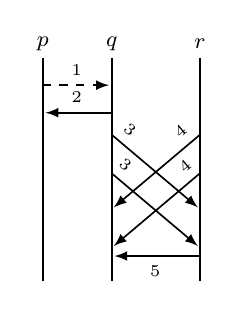
\begin{tikzpicture}[>=stealth,node distance=3.4cm,shorten >=1pt,
	  every state/.style={text=black, scale =0.6}, semithick,
		font={\fontsize{8pt}{12}\selectfont}]

	\begin{scope}[shift = {(8,0.75)}, scale = 0.7]
	  %MACHINES
	  \draw (0,1.25) node{$q$} ;
	  \draw (1.6,1.25) node{$r$} ;
	  \draw (-1.25,1.25) node{$p$} ;
	  \draw (0,1) -- (0,-3.1) ;
	  \draw (1.6,1) -- (1.6,-3.1);
	  \draw (-1.25,1) -- (-1.25,-3.1);

	  %MESSAGES
	  \draw[>=latex,->, dashed] (-1.25, 0.5) -- (0, 0.5) node[ above, midway] {$\amessage_1$};
	  \draw[>=latex,->] (0, 0) -- (-1.25, 0) node[ above, midway] {$\amessage_2$};


	  \draw[>=latex,->] (0, -0.4) -- (1.6, -1.75) node[pos=0.1, sloped, above] {$\amessage_3$};
	  \draw[>=latex,->] (0, -1.1) -- (1.6, -2.45) node[pos=0.05, sloped, above] {$\amessage_3$}; %{$\amessage_1'$};
	  %\draw[>=latex,->, dashed] (0, -2.5) -- (1.25, -3.25) node[pos=0.55, sloped, above] {$\amessage_1''$};

	  \draw[>=latex,->] (1.6, -0.4) -- (0, -1.75) node[pos=0.1, sloped, above] {$\amessage_4$};
	  \draw[>=latex,->] (1.6, -1.1) -- (0, -2.45) node[pos=0.05, sloped, above] {$\amessage_4$}; %{$\amessage_2'$};
	  %\node[rotate = 90, left]at (1.13, -0.65) {$\cdots$};
	  %\node[rotate = -90, right]at (0.1, -0.65) {$\cdots$};

	  \draw[>=latex,->] (1.6, -2.6) -- (0, -2.6) node[ below, midway] {$\amessage_5$};


	\end{scope}

	\end{tikzpicture}
	\captionof{figure}{MSC $\mscW$}
	\label{fig:msc_W}
	\end{center}
\end{minipage}

In \cite{BolligFG21} it is shown that, for the class of weakly synchronous MSCs, $SP$ is undecidable for $\comsymb = \oneone$, but decidable for $\comsymb = \oneone$.
Here we address the decidability of $SP$ for the class of weakly synchronous MSCs, considering also other communication models (these results are summarized in the second column of Fig.\ref{}). We now show that $SP$ is undecidable also for causally ordered communication. The proof is essentially identical to that given in \cite{BolligFG21} for the $\oneone$ case. We do the same reduction from the Post correspondence problem. The original proof considered a $\oneone$ system $\System$ with four machines (P1, P2, V1, V2), where we have unidirectional communication channels from provers (P1 and P2) to verifiers (V1 and V2). In particular notice that all the possible behaviours of $\System$ are causally ordered, i.e. $\ppL{\System} \subseteq \coMSCs$; according to how we built our system $\System$, it is impossible to have a pair of causally-related send events of P1 and P2\footnote{There is no channel between P1 and P2, and we only have unidirectional communication channels from provers to verifiers; it is impossible to have a causal path between two send events of P1 and P2.}, which implies that causal ordering is already ensured by any possible $\oneone$ behaviour of $\System$. The rest of the proof is identical to the $\oneone$ case.

\begin{proposition}\label{thm:co-weak-sync}
	The following problem is undecidable:
	Given finite sets $\Procs$ and $\Msg$ as well as a communicating system $\System$,
	is every MSC in $\coL{\System}$ weakly synchronous?
\end{proposition}

The hierarchy in Fig.~\ref{fig:msc_hierarchy_full} and the MSO formulas given in Section~\ref{sec:MSO} allow us to derive the decidability of $SP$ for the remaining communcation models.

\begin{proposition}\label{thm:weak-sync}
	Let $\comsymb \in \{$$\onen, $ $\nn\}$.
	The following problem is decidable:
	given finite sets $\Procs$ and $\Msg$ as well as a communicating system $\System$,
	is every MSC in $\cL{\System}$ weakly synchronous?
\end{proposition}
\begin{proof}
	We will consider $\comsymb = \onen$; the proof for $\comsymb = \nn$ follows the same steps. We would like to know if every MSC in $\onenL{\System}$ is in the class of weakly synchronous MSCs. Since every MSC in $\onenL{\System}$ is a $\onen$ MSC, we can equivalently restrict the problem to the class of weakly synchronous MSCs that are also $\onen$ MSCs. Let $\Class$ be the class of $\onen$ weakly synchronous MSCs; we show that $\Class$ is MSO-definable and STW-bounded, which implies the decidability of $SP$ for Theorem~\ref{thm:sync}. The class of weakly synchronous MSCs was shown to be MSO-definable in \cite{BolligFG21}; to be precise, their characterization is for $\oneone$ weakly synchronous MSCs (since their definition of MSC is equivalent to our definition of $\oneone$ MSC), but it also works for (asynchronous) weakly synchronous MSCs. We showed in Section~\ref{sec:MSO} that $\onenMSCs$ is MSO-definable; it follows that the class of $\onen$ weakly synchronous MSCs is also MSO-definable (we just take the conjuction of the the two formulas). The class of $\none$ weakly synchronous MSCs was shown to be STW-bounded in \cite{BolligFG21}, and since $\onenMSCs \subset \mbMSCs$, we also have that the class of $\none$ weakly synchronous MSCs has a bounded special treewidth. The claim follows from Theorem~\ref{thm:sync}.
\end{proof}

\subsection{Weakly \texorpdfstring{$k$}{k}-synchronous MSCs}

The undecidability result for some of the communication models motivates the study of other classes. Here we present weakly $k$-synchronous MSCs (\cite{BolligFG21}), which are a variant of weakly synchronous MSCs where the number of messages sent per exchange is at most $k$.

\begin{definition}[$k$-exchange]\label{def:weak-k-synchr}
Let $\msc = (\Events,\procrel,\lhd,\lambda)$ be an MSC
and $k \in \N$.
We call $\msc$ a $k$-\emph{exchange} if
$\msc$ is an exchange and $|\SendEv{\msc}| \le k$.
\end{definition}

\begin{definition}[weakly $k$-synchronous]\label{def:weaksync}
Let $k \in \N$.
We say that $\msc \in \MSCs$ is
weakly $k$-synchronous if it is of the form
$\msc = \msc_1 \cdot \ldots \cdot \msc_n$
such that every $\msc_i$ is a $k$-exchange.
\end{definition}

\noindent
\begin{minipage}[c]{10.5cm}
	\begin{example}
	MSC $\mscweakSexist$ in Fig.~\ref{fig:msc_weak_S_exist} is weakly $1$-synchronous, as it can be
	decomposed  into three \kE{1}s (the decomposition is depicted by the
	horizontal dashed lines). We remark that $\mscweakSexist \in
	\mbMSCs$. Note that there is a p2p linearization that respects the decomposition.
	On the other hand, a mailbox linearization needs to reorganize actions from different MSCs: the sending of
	$\msg_3$ needs to be done before the sending of $\msg_1$. Note that $\mscweakuniver$ in
	Fig.~\ref{fig:msc_weak_univer} is also weakly $1$-synchronous.
	\end{example}
\end{minipage}
	\hfill
\begin{minipage}[c]{3cm}
\begin{center}

	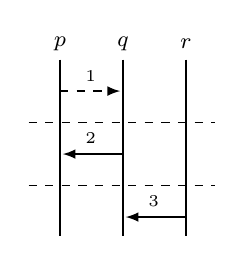
\begin{tikzpicture}[>=stealth,node distance=3.4cm,shorten >=1pt,
		every state/.style={text=black, scale =0.7}, semithick,
		font={\fontsize{8pt}{12}\selectfont}, scale = 0.8]

	  %MACHINES
	  \draw (0,0) node{$p$} ;
	  \draw (1,0) node{$q$} ;
	  \draw (2,0) node{$r$} ;
	  \draw (0,-0.25) -- (0,-3.1) ;
	  \draw (1,-0.25) -- (1,-3.1);
	  \draw (2, -0.25) -- (2, -3.1) ;
	  %MESSAGES
	  \draw[>=latex,->, dashed] (0,-0.75) -- (1, -0.75) node[midway,above]{$\amessage_1$};

	  \draw[>=latex,->] (1, -1.75) -- (0, -1.75) node[midway, above] {$\amessage_2$};
	  %\draw (0.5,-1.7) node{$\cdots$};
	  %\draw[>=latex,->] (1, -2.25) -- (0, -2.25) node[midway, above] {$\amessage_2$};

	  \draw[>=latex,->] (2,-2.75) -- (1,-2.75) node[midway, above] {$\amessage_3$};
	%\end{scope}
	  \draw[dashed] (-0.5,-1.25) -- (2.5,-1.25) ;
	  \draw[dashed] (-0.5,-2.25) -- (2.5,-2.25) ;


	\end{tikzpicture}
	\captionof{figure}{MSC $\mscweakSexist$}
	\label{fig:msc_weak_S_exist}

\end{center}
\end{minipage}

As for weakly synchronous MSCs, the class of weakly $k$-synchronous MSCs was already shown to be MSO-definable and STW-bounded in \cite{BolligFG21}, and these results still hold even for our definition of MSC. A direct application of Theorem~\ref{thm:sync} shows that, for weakly $k$-synchronous MSCs, $SP$ is decidable for all communication models.

\begin{proposition}\label{thm:weak-k-sync}
	Let $\comsymb \in \{$$\asy, $ $\oneone, $ $\co, $ $\none, $ $\onen, $ $\nn\}$.
	The following problem is decidable:
	given finite sets $\Procs$ and $\Msg$ as well as a communicating system $\System$,
	is every MSC in $\cL{\System}$ weakly $k$-synchronous?
\end{proposition}
\begin{proof}
	The class $\Class$ of weakly $k$-synchronous MSCs is MSO-definable and STW-bounded. $SP$ is decidable for Theorem~\ref{thm:sync}.
\end{proof}

\subsection{Existentially bounded MSCs}

We move now to existentially $k$-bounded MSCs, which have been studied extensively in literature \cite{DBLP:conf/fossacs/LohreyM02,DBLP:conf/dlt/GenestMK04,GKM07,BolligFG21}. These  kind of MSCs represent the behaviour of systems that can be realized with bounded channels, i.e. channels where at most $k$ messages can transit at any moment in time. For our definition of $k$-bounded MSCs, we suppose that there is a channel $(p,q)$ for any pair of processes such that $p$ sends messages to $q$ (there is a different channel for messages sent by $q$ to $p$). Intuitively, we say that an MSC is existentially $k$-bounded if it has linearization where, at any moment in time, there are no more than $k$ messages in any channel. Such a linearization will be referred to as a $k$-\emph{bounded linearization}. We give formal definitions below.

\begin{definition}\label{def:lin_k_bounded}
	Let $\msc = (\Events,\procrel,\lhd,\lambda) \in \MSCs$ and $k \in \N$.
	A linearization $\linrel$ of $\msc$ is called
	$k$-\emph{bounded} if, for all $e \in \SendEv{\msc}$, with $\lambda(e) = \sact{p}{q}{\msg}$, we have
	\[
	\sametype{e}{\pqsAct{p}{q}}{\linrel} - \sametype{e}{\pqrAct{p}{q}}{\linrel} \le k
	\]
\end{definition}
\noindent where $\sametype{e}{A}{\rel} = |\{f \in \Events \mid (f,e) \in \rel$ and $\lambda(f) \in A\}|$.
For instance, $\sametype{e}{\pqsAct{p}{q}}{\linrel}$ denotes the number of send events from $p$ to $q$ that occured before $e$ according to $\linrel$\footnote{Note that, since $\linrel$ in reflexive, $e$ itself is counted in $\sametype{e}{\pqsAct{p}{q}}{\linrel}$}.

\begin{definition}[Existentially bounded MSC]\label{def:ek_bounded_msc}
	Let $\msc = (\Events, \rightarrow, \lhd, \lambda) \in \asMSCs$ and $k \in \mathbb{N}$. We call $\msc$ \emph{existentially $k$-bounded} ($\exists k$-bounded) if it has a $k$-bounded linearization.
\end{definition}
We now look at the definitions of $\oneone$ $\exists k$-bounded MSCs and causally ordered $\exists k$-bounded, which are quite straightforward.

\noindent
\begin{minipage}[c]{10.5cm}
\begin{example}
  MSC $\mscexist$ in Fig.~\ref{fig:msc_exist}
  is existentially $1$-bounded, as witnessed by the linearization $!2\;!1\;!3\;?3\;?1\;!1\;?2\;!3\;?3 \ldots$
  Note that $\mscexist$ is not weakly synchronous as we cannot divide it into exchanges.
\end{example}
\end{minipage}
\begin{minipage}[c]{3cm}
	\begin{center}
		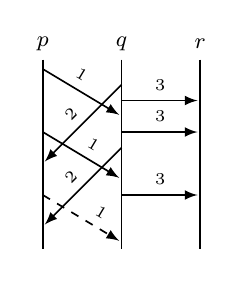
\begin{tikzpicture}[>=stealth,node distance=3.4cm,shorten >=1pt,
		every state/.style={text=black, scale =0.7}, semithick,
		  font={\fontsize{8pt}{12}\selectfont}]
	  \begin{scope}[shift = {(0,0)}, scale = 0.8]
		% \draw (1.25, -4.75) node{\textbf{(a)}};
		% \draw (4.5, -4.75) node{\textbf(b)};

		%MACHINES
		\draw (0,-0.1) node{$p$} ;
		\draw (1.25,-0.1) node{$q$} ;
		\draw (2.5,-0.1) node{$r$} ;
		\draw (2.5, -0.35) -- (2.5, -3.4) ;
		\draw (0,-0.35) -- (0,-3.4) ;
		\draw (1.25,-0.35) -- (1.25,-3.4);
		%MESSAGES

		\draw[>=latex,->] (0, -0.5) -- (1.25, -1.25) node[pos=0.4, sloped, above] {$\amessage_1$};
		\draw[>=latex,->] (0, -1.5) -- (1.25, -2.25) node[pos=0.55, sloped, above] {$\amessage_1$};
		\draw[>=latex,->, dashed] (0, -2.5) -- (1.25, -3.25) node[pos=0.65, sloped, above] {$\amessage_1$};

		\draw[>=latex,->] (1.25, -0.75) -- (0, -2) node[pos=0.5, sloped, above] {$\amessage_2$};
		\draw[>=latex,->] (1.25, -1.75) -- (0, -3) node[pos=0.5, sloped, above] {$\amessage_2$};


		\draw[>=latex,->] (1.25, -1) -- (2.5, -1) node[midway, above] {$\amessage_3$};
		\draw[>=latex,->] (1.25, -1.5) -- (2.5, -1.5) node[midway, above] {$\amessage_3$};
		\draw[>=latex,->] (1.25, -2.5) -- (2.5, -2.5) node[midway, above] {$\amessage_3$};

		%\draw (0.6, -3.35) node{$\cdots$};
		%\draw (1.9, -3.35) node{$\cdots$};
	  \end{scope}
			% \begin{scope}[shift = {(3,0)}, scale = 0.8]
			%   % \draw (0.5, -4) node{\textbf{(b)}};
			%   %MACHINES
			%   \draw (0,0) node{$p$} ;
			%   \draw (1,0) node{$q$} ;
			%   \draw (0,-0.25) -- (0,-3.5) ;
			%   \draw (1,-0.25) -- (1,-3.5);
			%   %MESSAGES
			%
			%    \draw[>=latex,->] (0, -0.75) -- (1, -0.75) node[midway, above] {$\amessage_1$};
			%    \draw[>=latex,->] (1, -1.5) -- (0, -1.5) node[midway, above] {$\amessage_2$};
			%    \draw[>=latex,->] (0, -2.25) -- (1, -2.25) node[midway, above] {$\amessage_1$};
			%    \draw[>=latex,->] (1, -3) -- (0, -3) node[midway, above] {$\amessage_2$};
			%
			%
			%   % \draw (0.5, -3.25) node{$\cdots$};
			% \end{scope}
			  \end{tikzpicture}
	  \captionof{figure}{MSC $\mscexist$}
	  \label{fig:msc_exist}
	\end{center}
\end{minipage}

\begin{definition}
	An MSC $\msc$ is \emph{$\oneone$ existentially $k$-bounded} ($\oneone$-$\exists k$-bounded) if it is a $\oneone$ MSC and it is also existentially $k$-bounded.
\end{definition}
\begin{definition}
	An MSC $\msc$ is \emph{causally orderered existentially $k$-bounded} ($\cosymb$-$\exists k$-bounded) if it is a causally ordered MSC and it is also existentially $k$-bounded.
\end{definition}

When moving on to the other communication models, the definitions are not as straightforward. For instance, the definition of $\none$ $\exists k$-bounded MSC should require that there exists a $k$-bounded linearization that is also a $\none$ linearization, not just any linearization. Recall that an MSC is a $\none$ MSC if it has at least one $\none$ linearization, which represents a sequence of events that can be executed by a $\none$ system. Following this intuition, we want one of these $\none$ linearizations to be $k$-bounded, not just any linearization.

\begin{definition}
	An MSC $\msc$ is \emph{$\none$ existentially $k$-bounded} ($\none$-$\exists k$-bounded) if it has a $k$-bounded $\none$ linearization.
\end{definition}
% \davide{This paragraph depends on how we choose to formally define the mailbox communication model... we could go for a (i) single incoming channel, or (ii) just an enforcing of the delivery of messages by the transport layer.}
% It should be noted that, for a $k$-bounded mailbox linearization, it is not necessarily true that at any time we have at most $k$ messages in each channel. Recall that in the mailbox communication architecture every process has a single incoming channel, but the Definition~\ref{def:lin_k_bounded} of $k$-bounded linearization considers the number of pending messages between each pair $(p,q)$ of processes. Let $n$ be the number of processes. We can say that, for a $k$-bounded mailbox linearization, we have at most $k(n-1)$ messages in each channel at any moment (because each process can have at most $k$ pending messages coming from any of the other $n-1$ processes).
% \davide{An example would be nice.}

\begin{definition}
	An MSC $\msc$ is \emph{$\onen$ existentially $k$-bounded} (onen-$\exists k$-bounded) if it has a $k$-bounded $\onen$ linearization.
\end{definition}

\begin{definition}
	An MSC $\msc$ is \emph{$\nn$ existentially $k$-bounded} (nn-$\exists k$-bounded) if it has a $k$-bounded $\nn$ linearization.
\end{definition}

We show that each of the $\exists k$-bounded classes of MSCs presented so far is MSO-definable and STW-bounded. We then derive the decidability of $SP$ in a similar way to what we did in the proof of Proposition~\ref{thm:weak-sync} for weakly synchronous MSCs.

\paragraph*{MSO-definability}

Here we will investigate the MSO-definability of all the variants of $\exists k$-bounded MSCs, starting from the most general class of $\exists k$-bounded MSCs.
Following the approach taken in \cite{DBLP:conf/fossacs/LohreyM02}, we introduce a binary relation $\relb$ ($\linrel_b$ in their work) associated with a given bound $k$ and an MSC $\msc$. Let $k \ge 1$ and $\msc$ be a fixed MSC: we have $r \relb s$ if, for some $i \ge 1$ and some channel ($p$,$q$)\footnote{Recall that ($p,\,q$) is a channel where messages are sent by $p$ and received by $q$.}:
\begin{enumerate}\itemsep=0.5ex
	\item $r$ is the $i$-th receive event (executed by $q$).
	\item $s$ is the ($i+k$)-th send event (executed by $p$).
\end{enumerate}
Note that, for any two events $s$ and $r$ such that $r \relb s$, every linearization of $\msc$ in which $r$ is executed after $s$ cannot be $k$-bounded. Intuitively, we can read $r \relb s$ as "$r$ has to be executed before $s$ in a $k$-bounded linearization". A linearization $\linrel$ that respects $\relb$ (i.e. $\relb \,\subseteq\, \linrel$) is $k$-bounded.\davide{An example could be nice.} In \cite{DBLP:conf/fossacs/LohreyM02} it was shown that an MSC is $\exists k$-bounded if and only if the relation $\le_\msc \cup \relb$ is acyclic. Since $\le_\msc$ and acyclicity are both MSO-definable, it suffices to find an MSO formula that defines the $\relb$ relation to claim the MSO-definability of $\exists k$-bounded MSCs. Unfortunately, $\relb$ is not MSO-definable because MSO logic cannot be used to "count" for an arbitrary $i$. For this reason, we introduce a similar MSO-definable binary relation $\relbAsy$, and we show that an MSC $\msc$ is $\exists k$-bounded MSC iff $\le_\msc \cup \relbAsy$ is acyclic and another condition holds. Let $k \ge 1$ and $\msc$ be a fixed MSC; we have $r \relbAsy s$ if, for some $i \ge 1$ and some channel ($p$,$q$):
\begin{itemize}\itemsep=0.5ex
	\item There are $k+1$ send events $(s_1, \dots, s_k, s)$, where at least one is matched, such that $s_1 \procrel^+ \dots \procrel^+ s_k \procrel^+ s$.
 	\item $r$ is the first receive event for the matched send events among $s_1, \dots, s_k, s$.
\end{itemize}

\begin{proposition}\label{prop:asy_ek_def_alt}
	An MSC $\msc$ is $\exists k$-bounded if and only if $\le_\msc \cup \relbAsy$ is acyclic and, for each channel ($p$,$q$), there are at most $k$ unmatched send events.
\end{proposition}
\begin{proof}
	($\Rightarrow$) Suppose $\msc$ is $\exists k$-bounded, which by definition means there is at least one $k$-bounded linearization $\linrel$. Firstly, notice that every MSC that has more than $k$ unmatched send events in any channel cannot be an $\exists k$-bounded MSC. We already know that $\le_\msc \subseteq \linrel$, and we will show show that also $\relbAsy \subseteq \linrel$. This implies that $\le_\msc \cup \relbAsy$ is acyclic, otherwise we would not be able to find a linearization $\linrel$ that respects both $\le_\msc$ and $\relbAsy$. Suppose, by contradiction, that $\relbAsy \nsubseteq \linrel$, i.e. there are two events $r$ and $s$ such that $r \relbAsy s$ and $s \linrel r$. By definition of $\relbAsy$, there are $k$ send events in a channel ($p$,$q$) that are executed before $s$, and whose respective receive events happens after $r$. If $s$ is executed before $r$ in the linearization, there will be $k+1$ messages in channel (i.e. $\linrel$ is not a $k$-bounded linearization). We reached a contradiction, hence $\relbAsy \subseteq \linrel$ and $\le_\msc \cup \relbAsy$ is acyclic.\newline
	($\Leftarrow$) Suppose $\le_\msc \cup \relbAsy$ is acyclic and, for each channel ($p$,$q$), there are at most $k$ unmatched send events. If $\le_\msc \cup \relbAsy$ is acyclic, we are able to find at least one linearization $\linrel$ for the partial order $(\le_\msc \cup \relbAsy)^\ast$. We want to show that this linearization is $k$-bounded. By contradiction, suppose $\linrel$ is not $k$-bounded, i.e. we are able to find $k+1$ send events $s_1 \procrel^+ \dots \procrel^+ s_k \procrel^+ s$ on a channel ($p$,$q$), such that $s$ is executed before any of the respective receive events takes place. There are two possible scenarios:
	\begin{itemize}\itemsep=0.5ex
		\item Suppose all the $k+1$ send events are unmatched. This is impossible, since we supposed that there are at most $k$ unmatched send events for any channel.
		\item Suppose there is at least one matched send event between the $k+1$ sends. Let the first matched send event be $s_i$ and let $r$ be the receive event that is executed first among the receive events for these $k+1$ sends. By hypothesis, $s \linrel r$. However, according to the definition of $\relbAsy$, we must have $r \relbAsy s$. We reached a contradiction, since we cannot have that $s$ happens before $r$ in a linearization for the partial order $(\le_\msc \cup \relbAsy)^\ast$, if $r \relbAsy s$.
	\end{itemize}
\end{proof}

\noindent According to Proposition~\ref{prop:asy_ek_def_alt}, we can write the MSO formula the defines $\exists k$-bounded MSCs as
\[
\Psi_{\exists k}=
acyclic(\le_\msc \cup \relbAsy) \;\wedge\;
\neg \left(
	\exists s_1 \dots s_{k+1}. s_1 \procrel^+ \dots \procrel^+ s_{k+1} \;\wedge \;
	allSends\_p\_q(k+1) \;\wedge\; allUnm
\right)
\]
\[
allSends\_p\_q (t) =
\bigvee_{\substack{p \in \Procs, q \in \Procs}}\;
\bigwedge_{s \in {s_1, ..., s_{t}}}\;
\bigvee_{a \in \pqsAct{p}{q}}
(\lambda(s) = a)
\]
\[
allUnm = \bigwedge_{s \in {s_1, ..., s_{k+1}}}(\neg \mathit{matched}(s))
\]
where $acyclic(\le_\msc \cup \relbAsy)$ is an MSO formula that checks the acyclicity of $\le_\msc \cup \relbAsy$, and the $\relbAsy$ relation can be defined as
\[
r \relbAsy s= \exists s_1 \dots s_{k+1}. \left(
\begin{array}{rl}
	& s_1 \procrel^+ \dots \procrel^+ s_{k+1} \;\wedge\;
	allSends\_p\_q(k+1) \;\wedge\; \\
	& \exists r. (\bigvee_{s \in {s_1, ..., s_{k+1}}}s \lhd r) \;\wedge\;
	\bigwedge_{e \in {s_1, ..., s_{k+1}}}(\exists f.e \lhd f \implies r \procrel^* f) \\
\end{array}
\right)
\]

\medskip

It follows that, given $k \in \N$, the set of existentially $k$-bounded MSCs is MSO-definable. Causally ordered and $\oneone$ existentially $k$-bounded MSCs are clearly MSO-definable by definition, since we already showed that $\oneone$ MSCs, causally ordered MSCs, and existentially $k$-bounded MSCs are all MSO-definable. Recall that we introduced the $\relbAsy$ relation because the $\relb$ relation introduced in \cite{DBLP:conf/fossacs/LohreyM02} was not MSO-definable for asynchronous communication. However, when considering $\oneone$ communication\footnote{And also all of the other communication models, because of the hierarchy shown in Section~\ref{sec:hierarchy}}, $\relb$ becomes MSO-definable; the FIFO behaviour ensures that, for any channel $(p,q)$, the $i$-th matched send event of $p$ matches with the $i$-th receive event of $q$. This allows us to define $r \relb s$ as:
\[
r \relb s=\exists s_1. \dots \exists s_k.\left(
allSends\_p\_q(k)
\;\wedge\; s_1\procrel s_2\procrel\dots
\procrel s_k\procrel s
\;\wedge\; s_1 \lhd r
\right)
\]
Recall that an MSC $\msc$ is $\none$-$\exists k$-bounded if has a linearization that is both $\none$ and $\exists k$-bounded. A linearization $\linrel_\msc$ is $\none$ if $\msc$ is $\none$ and $\linrel_\msc$ is a linear extension of the partial order $\preceq_\msc$, i.e. $\preceq_\msc \;\subseteq\; \linrel_\msc$. A linearization $\linrel_\msc$ is $\exists k$-bounded if $\relb \;\subseteq\; \linrel_\msc$. It follows that a linearization $\relb$ is $\none$-$\exists k$-bounded if $(\preceq_\msc \cup \relb) \;\subseteq\; \linrel_\msc$. Such a linerization exists only if $\preceq_\msc \cup \relb$ is acyclic\footnote{If $\preceq_\msc \cup \relb$ is acyclic, its transive closure always exists and it is a partial order, hence we are always able to find a linear extension.}. The characterization for onen-$\exists k$-bounded MSCs and nn-$\exists k$-bounded is very similar. Below the formal definitions.

\begin{proposition}\label{prop:ek-mso}
	An MSC $\msc$ is $\none$-$\exists k$-bounded iff the relation $\preceq_\msc \cup \relb$ is acyclic.\\
	An MSC $\msc$ is onen-$\exists k$-bounded iff the relation $\lessdot_\msc \cup \relb$ is acyclic.\\
	An MSC $\msc$ is nn-$\exists k$-bounded iff the relation $\bowtie_\msc \cup \relb$ is acyclic.
\end{proposition}

The MSO-definability of all the variants of $\exists$k-bounded MSCs directly follows from Prop.~\ref{prop:ek-mso}, since all of these relations were shown to be MSO-definable.

\paragraph*{Special treewidth}

In \cite[Lemma 5.37]{DBLP:journals/corr/abs-1904-06942} it was shown that the special treewidth of existentially $k$-bounded MSCs is bounded by $k\,|\Procs|^2$, for $k \ge 1$. Actually, STW-boundness was shown for the more general class of Concurrent Behaviours with Matching ($\mathsf{CBM}$), but the result is still valid since $\asMSCs \subset \mathsf{CBM}$. The special treewidth of the other classes of $\exists k$-bounded MSCs is also bounded, since they are clearly subclasses of $\exists k$-bounded MSCs.

\subsection{Universally bounded MSCs}

An MSC is existentially $k$-bounded if it has a $k$-bounded linearization. We call an MSC universally $k$-bounded MSCs if all of its linearizations are $k$-bounded, hence the name "universally".

\begin{definition}[Universally bounded MSC]\label{def:uk_bounded_msc}
	Let $\msc = (\Events, \rightarrow, \lhd, \lambda) \in \asMSCs$ and $k \in \mathbb{N}$. We call $\msc$ \emph{universally $k$-bounded} ($\forall k$-bounded) if all of its linearizations are $k$-bounded.
\end{definition}
\begin{definition}
	An MSC $\msc$ is \emph{\pp universally $k$-bounded} (\pp-$\forall k$-bounded) if it is a \pp MSC and it is also universally $k$-bounded.
\end{definition}
\begin{definition}
	An MSC $\msc$ is \emph{causally orderered universally $k$-bounded} ($\cosymb$-$\forall k$-bounded) if it is a causally ordered MSC and it is also universally $k$-bounded.
\end{definition}

As for the existential case, the definitions for the other communication models are not as straightforward. For instance, the definition of $\none$ $\forall k$-bounded MSC should require that all the $\none$ linearizations of the MSC are $k$-bounded, but we say nothing about linearizations that are not $\none$. The same goes for the $\onen$ and $\nn$ communication models.

\begin{definition}
	An MSC $\msc$ is \emph{mailbox universally $k$-bounded} (mb-$\forall k$-bounded) if it is a mailbox MSC and all of its mailbox linearizations are $k$-bounded.
\end{definition}
\begin{definition}
	An MSC $\msc$ is \emph{$\onen$ universally $k$-bounded} (1n-$\forall k$-bounded) if it is a $\onen$ MSC and all of its $\onen$ linearizations are $k$-bounded.
\end{definition}

% \subsubsection{Hierarchy}

% \davidequestion{I think that this section, albeit interesting, might be removed...}
% In this section we will investigate the relations between the various classes of universally $k$-bounded MSCs that we introduced. From their definition, it is quite straightforward to see that $\coUk \subseteq \ppUk \subseteq \asUk$. The set of mailbox universally $k$-bounded MSCs, however, does not fit in this hierarchy. Recall that an MSC is mb-$\forall k$-bounded if all of its mailbox linearizations are $k$-bounded, but the definition does not say anything about non-mailbox linearizations. It can be the case that an MSC has a bound $k$ for its mailbox linearizations, but a higher bound $k'$ for non-mailbox linearizations. Fig.~\ref{fig:mb_uk} shows an MSC $\msc$ which is mb-$\forall 1$-bounded, but $\forall 2$-bounded. According to the mailbox semantics, a mailbox linearization of $\msc$ has to respect the order $!m_1 \mbrel_\msc\, !m_3 \mbrel_\msc\, !m_4$. Note that all mailbox linearizations are $1$-bounded, but we are able to find a non-mailbox linearization that is 2-bounded, such as $!m_1 \linrel\, !m_4 \linrel\, ?m_1 \linrel\, !m_2 \linrel\, ?m_2 \linrel\, !m_3 \linrel\, !m_4 \linrel\, ?m_3 \linrel\, ?m_4$.

% \begin{figure}[h]
% \begin{center}
% \begin{tikzpicture}
% 	\newproc{0}{p}{-1.9};
% 	\newproc{1}{q}{-1.9};
% 	\newproc{2}{r}{-1.9};

% 	\newmsgml{0}{1}{-0.5}{1}{0.5}{black};
% 	\newmsgml{1}{2}{-0.7}{2}{0.5}{black};
% 	\newmsgml{2}{1}{-1.2}{3}{0.5}{black};
% 	\newmsgml{0}{1}{-1.4}{4}{0.5}{black};
% \end{tikzpicture}
% \caption{Example of MSC which is mailbox universally 1-bounded, but not universally 1-bounded (it is universally 2-bounded).}
% \label{fig:mb_uk}
% \end{center}
% \end{figure}

% For a given $k \in \N$, Fig~\ref{fig:uk_hierarchy} gives a visual representation of how the diffent variants of universally $k$-bounded MSCs are related.

% \begin{figure}[h]
% 	\centering
% 	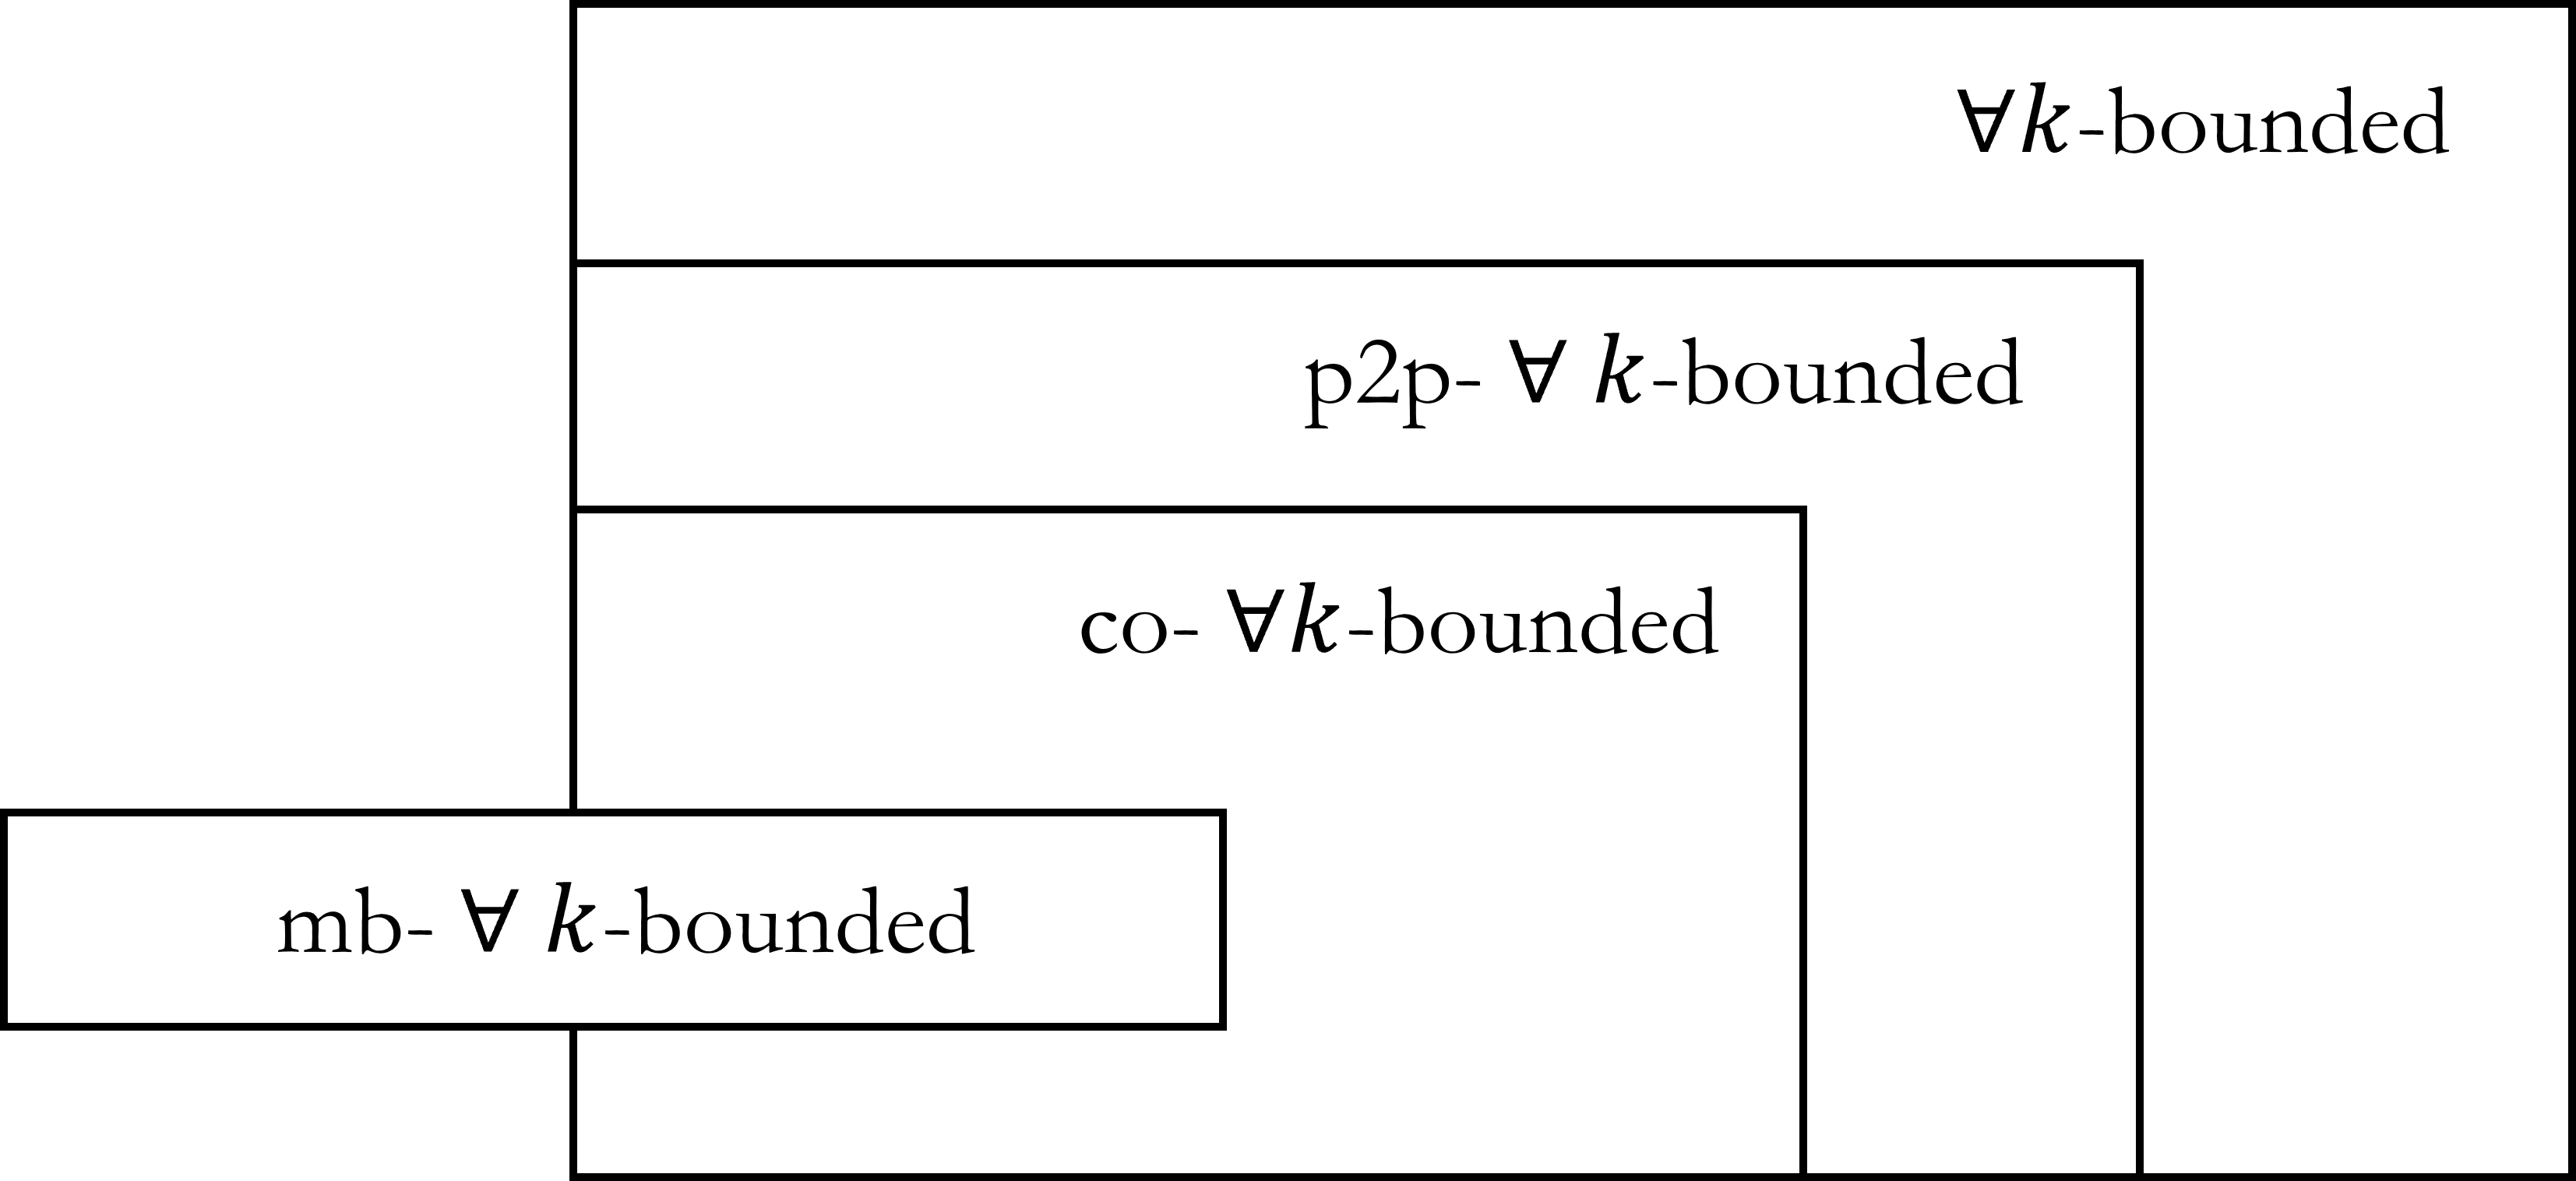
\includegraphics[width=8cm]{uni_k_hierarchy.png}
% 	\caption{The relation between different variants of universally $k$-bounded MSCs, given a $k \in \N$.}
% 	\label{fig:uk_hierarchy}
% \end{figure}

\paragraph*{MSO-definability}

In this section, we will investigate the MSO-definability of all the variants of universally $k$-bounded MSCs that we discussed.
In \cite{DBLP:conf/fossacs/LohreyM02}, it is shown that an MSC $\msc$ is universally $k$-bounded if and only if $\relb \;\subseteq\; \le_\msc$. In other words, $r \relb s \Rightarrow r \le_\msc s$ for any two events $r$ and $s$. This is equivalent to saying that every linearization $\linrel$ of $\msc$ respects the $\relb$ relation, since $\relb \;\subseteq\; \le_\msc \;\subseteq\; \linrel$. We already saw that $\relb$ is not MSO-definable when communication is asynchronous, hence we will use the $\relbAsy$ relation to give the following alternative characterization of universally $k$-bounded MSCs.

\begin{proposition}
	An MSC $\msc$ is $\forall k$-bounded if and only if $\relbAsy \;\subseteq\; \le_\msc$ and, for each channel ($p$,$q$), there are at most $k$ unmatched send events.
\end{proposition}
\begin{proof}
	($\Rightarrow$) Suppose $\msc$ is $\forall k$-bounded, which by definition means that all of its linearization are $k$-bounded. Firstly, notice that every MSC that has more than $k$ unmatched send events in any channel cannot be an $\forall k$-bounded MSC (not even $\exists k$-bounded). By contradiction, suppose that $\relbAsy \;\nsubseteq\; \le_\msc$, i.e. there are two events $r$ and $s$ such that $r \relbAsy s$ and $r \nleq_\msc s$. If $r \nleq_\msc s$, we either have that $s \le_\msc r$ or that $s$ and $r$ are incomparable w.r.t. $\le_\msc$; note that, in both cases, $\msc$ must have one linearization where $s$ happens before $r$\footnote{If two elements $a$ and $b$ of a set are incomparable w.r.t. a partial order $\le$, it is always possible to find a total order of the elements (that respects $\le$) where $a$ comes before $b$, or viceversa.}. The existence of such a linearization implies that $\msc$ is not $\forall k$-bounded.
	($\Leftarrow$) Suppose $\relbAsy \;\subseteq\; \le_\msc$ and, for each channel ($p$,$q$), there are at most $k$ unmatched send events. By definition, every linearization $\linrel$ of $\msc$ is such that $\le_\msc \;\subseteq\; \linrel$; it follows that $\relbAsy \;\subseteq\; \linrel$, which means that every linearization of $\msc$ is $k$-bounded, i.e. $\msc$ is $\forall k$-bounded.
\end{proof}

It follows that $\oneone$-$\forall k$-bounded and $\co$-$\forall k$-bounded MSCs are MSO-definable by definition, since $\oneone$ MSCs, causally ordered MSCs, and universally $k$-bounded MSCs are all MSO-definable. We already showed that $\relb$ is MSO-definable when considering $\oneone$ communication. The characterization for the other communication models is similar to that given in \cite{DBLP:conf/fossacs/LohreyM02}, but it uses the proper relation for each communication model.

\begin{proposition}\label{prop:mb_ukb_alt}
	An MSC $\msc$ is $\none$-$\forall k$-bounded if and only if $\relb \;\subseteq\; \preceq_\msc$.\\
	An MSC $\msc$ is onen-$\forall k$-bounded if and only if $\relb \;\subseteq\; \lessdot_\msc$.\\
	An MSC $\msc$ is nn-$\forall k$-bounded if and only if $\relb \;\subseteq\; \bowtie_\msc$.
\end{proposition}
\begin{proof}
	We only show it for the $\none$ communication model. The proof for the other communication models works the same way. Consider an MSC $\msc$ and a $k \in \N$.\newline
	($\Leftarrow$) Suppose $\relb \;\subseteq\; \preceq_\msc$. For every mailbox linearization $\linrel$ of $\msc$ we have that $\preceq_\msc \;\subseteq\; \linrel$. This implies $\relb \;\subseteq\; \linrel$, that is to say every mailbox linearization is $k$-bounded.\newline
	($\Rightarrow$) Suppose $\msc$ is a $\none$-$\forall k$-bounded MSC. By definition, every mailbox linearization $\linrel$ of $\msc$ is $k$-bounded, i.e. $\relb \;\subseteq\; \linrel$, and we have $\preceq_\msc \;\subseteq\; \linrel$, according to the definition of mailbox linearization. Moreover, we also know that $\preceq_\msc \cup \relb$ is acyclic, since $\msc$ is $\exists k$-bounded\footnote{Every $\none$-$\forall k$-bounded MSC is also a $\none$-$\exists k$-bounded MSC by definition.}. Suppose now, by contradiction, that $\relb \;\nsubseteq\; \preceq_\msc$. Thus, there must be at least two events $r$ and $s$ such that $r \relb s$ and $r \npreceq_\msc s$; we also have $s \npreceq_\msc r$ because of the acyclicity of $\preceq_\msc \cup \relb$ (we cannot have the cycle $r \relb s \preceq_\msc r$). Consider a mailbox linearization $\linrel$  of $\msc$, such that $s \linrel r$. Note that such a mailbox linearization always exists, since $r$ and $s$ are incomparable w.r.t. the partial order $\preceq_\msc$. This mailbox linearization does not respect $\relb$ (because we have $s \linrel r$ and $r \relb s$), so it is not $k$-bounded. This is a contradiction, since we assumed that $\msc$ was a $\none$-$\forall k$-bounded MSC. It has to be that $\relb \;\subseteq\; \preceq_\msc$.
\end{proof}

Using Proposition~\ref{prop:mb_ukb_alt}, we can now easily write the MSO formulas that defines these variants of universally $k$-bounded MSCs.
\begin{align*}
	\mbUkformula &= \neg \exists r.\exists s.(r \relb s \wedge \neg(r \preceq_\msc s)) \\
	\onenUkformula &= \neg \exists r.\exists s.(r \relb s \wedge \neg(r \lessdot_\msc s)) \\
	\nnUkformula &= \neg \exists r.\exists s.(r \relb s \wedge \neg(r \bowtie_\msc s))
\end{align*}


\paragraph*{Special treewidth}

All the variants of universally $k$-bounded MSCs that we presented have a bounded special treewidth. This directly follows from the STW-boundness of the existential counterparts, since every universally $k$-bounded MSC is existentially $k$-bounded by definition.
